\chapter{
Modeling Space Usage: 
Integrating Resource Selection Information with 
Spatial Capture-Recapture
  Models}

\markboth{Chapter XXX}{}
\label{chapt.rsf}


\vspace{.3in}

Up to this point we have developed many specific variations of
relatively simple SCR models. They included various models of the
observation process, 
models of the relationship between encounter probability and distance,
and different types of
covariates including behvioral responses and other things that should
affect detection probability.  That said, the models remain pretty
basic in the sense that they imply simplistic models of how
individuals use space (section \ref{scr0.sec.implied}) and how individuals are
distributed in space.  In the following several chapters we generalize
some of the core SCR assumptions to accommodate more realistic notions
of how animals use space.

In this chapter we extend our notion of encounter probability models
as models of resource selection (sec. \ref{scr0.sec.implied}), by
extending them to included explicit landscape covariates. We do this
in a way that is entirely consistent with the manner in which
classical ``resource selection function'' (RSF) models are estimated
from animal telemetry data.  In fact, we argue there that SCR models
and ``RSF/telemetry'' models have the same basic underlying model of
space usage, just that in the SCR model encounter of individuals is
imperfect (i.e., $p<1$) whereas RSF data obtained by telemetry is
perfect (i.e., p=1). We can think of the two as being exactly
equivalent either if we have a dense array of trapping devices, or if
our telemetry apparatus is imperfect (fails a large percentage of the
time, randomly).  A key conceptual thing is we need to formulate both
the SCR model and the RSF model in terms of a common latent variable
so that we can make them consistent with respect to some underlying
space utilization process.


Here we show how to integrate standard RSF type data into SCR models
to model space usage expcliitly. This produces asymmetric, irregular
and non-stationary home ranges, and allows us to make formal
inferences about factors that influence home range geoemetry and
morphology directly from SCR data.  We begin by describing a model for
space usage that exists independent of how we obtain the data. Then we
introduce observation models consistent with both standard
capture-recapture methods and telemetry.  This allows us to define a
general likeleihood function that is the product of the two
components, if they are both simultaneously available.  In the absence
of RSF data from telemetry, the model reduces to an ordinary SCR model
but with a spatial covariate on encounter probability.  In summary,
the framework allows us to estimate RSFs directly from SCR data, or to
integrate telemetry data directly into SCR models.

XXXX below par goes elsewhgere XXXXX

In our formulation we estimate the latent ${\bf s}$ variables from the observed telemetry
data, just as a convenience, but this wouldn't be necessary.
Also we assume the data are independent pieces but if some of the SCR
individuals are the same as the telemetered individuals then we should
probably account for that explicitly. So right now we pretend we don't
know anything about the telemtered guys in terms of their capture
history. So they don't contribute to information about baseline
encounter probability, just to estimates of the other encounter model
parameters. 



\section{Basic Model of Space Usage}

We devevlop the model here in terms of a discrete landscape purely for
computational expediency. That said, essentially no landscape on your
computer is continuous, the one exception is if the landscape is
defined strictly in terms of variables that themselves are inherently
continuous -- e.g., ``distance to road'' or something like that.  But
almost all habitat or landscape structure data comes to us in the form
of raster data.  Let $x_{1},\ldots,x_{nG}$ identify the center
coordinates of a set of $nG$ pixels that define a landscape. ({\bf
  consistent with other notation?}) We organize them into a matrix
${\bf X}_{nG \times 2}$. 
Let $z(x)$ denote a covariate defined for every pixel $x$. 

We suppose that a population of individuals wanders around space in
some manner related to the covariate $z(x)$, and their locations
accumulate in pixels by some omnipotent accounting mechanism. Let
$n_{ij}$ be the number of times individual $i$ used pixel $j$ during
some period of time. 
We assume the
following probability mass function 
for the distribution of  ``use'' -- the number of
occurrences of individual $i$ in pixel $j$:
\[
{\bf n}_{i} \sim \mbox{Multinom}({\bm \pi}_{i})
\]
where
\[
 \pi_{ij} = \frac{ exp( -\alpha_{2} z(x) ) }{ \sum_{x} exp(-\alpha_{2} z(x))} 
\]
This is the standard RSF
model XXXX REFS XXXXXX used to model telemetry data. 
In practice, we don't get to observe $n_{ij}$ for all individuals but,
instead, only for a small subset which we capture and install
telemetry devices on.
For these telemetered individuals
we accumulate individual- and pixel-specific frequencies,
 at a lower sampling rate than actual individual use. For
example, we might choose to record the location of an individual every
hour or day or whatever. As such, the observed frequency of pixel use
is a sample but, if the recording is random or systematic (or
otherwise unrelated to {\it where} individuals are located), then we
can imagine that the same model of space usage applies. (formally, we
suppose that the observed frequencies are a binomial sample with
sample size $n_{ij}$ and sampling intensity $\alpha_{0}$ lets say, and
we see that the constant $\alpha_{0}$ cancels from the expression for
the multinomoial cell probabilities above). 

For the telemtered individuals then, 
we addopt the standard RSF
model  which has probabilities as above:
\[
 \pi_{i,j} = \frac{ exp( -\alpha_{2} z(x) ) }{ \sum_{x} exp(-\alpha_{2} z(x))} 
\]
We could have multiple such covariates but we focus on a
single covariate here for clarity.  We extend this model slightly to
make it more realistic spatially. Let ${\bf s}$ denote the centroid of
an individuals home range and let $D_{ij}$ be the distance from ${\bf
  s}_{i}$ to pixel ${\bf x}_{j}$. We modify the space usage model to
accomodate that space use will be concentrated 
around an individuals home range centroid:
\[
 \pi_{i,j} = \frac{ exp( -\alpha_{1} D_{ij}^{2} -\alpha_{2} z(x) ) }
{ \sum_{x} exp(-\alpha_{1} D_{ij}^{2} -\alpha_{2} z(x))} 
\]
In this case, if you have no covariates at all, or if $\alpha_{2} =
0$, then 
the probabilities $\pi_{ij}$ are directly proportional to the SCR
model for encounter probability.
For example, setting $\alpha_{2} = 0$, then this implies probability
of use for pixel $j$ is:
\[
p_{ij} \propto  exp( -\alpha_{1} D_{ij}^{2})
\]
so whatever function of distance we use in our RSF implies an
equivalent model of space usage when used in SCR models. 

As an illustration of space usage patterns under this model, we
simulated a covariate that we feel represents typical habitat
structure (Fig. \ref{rsf.fig.habitat}). This was simulated by using a
basic kriging model with the following commands:
\begin{verbatim}
set.seed(1234)
gr<-make.grid(minx=1,maxx=40,miny=1,maxy=40,nx=40,ny=40)
Dmat<-as.matrix(dist(gr))
V<-exp(-Dmat/5)
z<-t(chol(V))%*%rnorm(1600)
spatial.plot(gr,z)
\end{verbatim}
The functions \mbox{\tt make.grid} and \mbox{\tt spatial.plot} are
both in the \mbox{\tt scrbook} package.
We show an example of space usage for 8 individuals ....... in
Fig. \ref{rsf.fig.homeranges},
simulated with $\alpha_{1} = 1/(2\sigma^2)$ with $\sigma = 2$ and the
coefficient on $z(x)$ set to $\alpha_{2} = 1$. 
These exhibit clear non-stationarity in
response to the structure of the underlying covariate 
and are distinctly asymmetrical.  We noet that if $\alpha_{2}$ were
set to 0, the 8 home ranges shown here would equate precisely to
bivariate normal kernels with $\sigma = 2$. 
An interesting thing to note is that the activity centers are not
typically located in the pixel of highest use or even the centroid of
usage. 

\begin{figure}[htp]
\centering
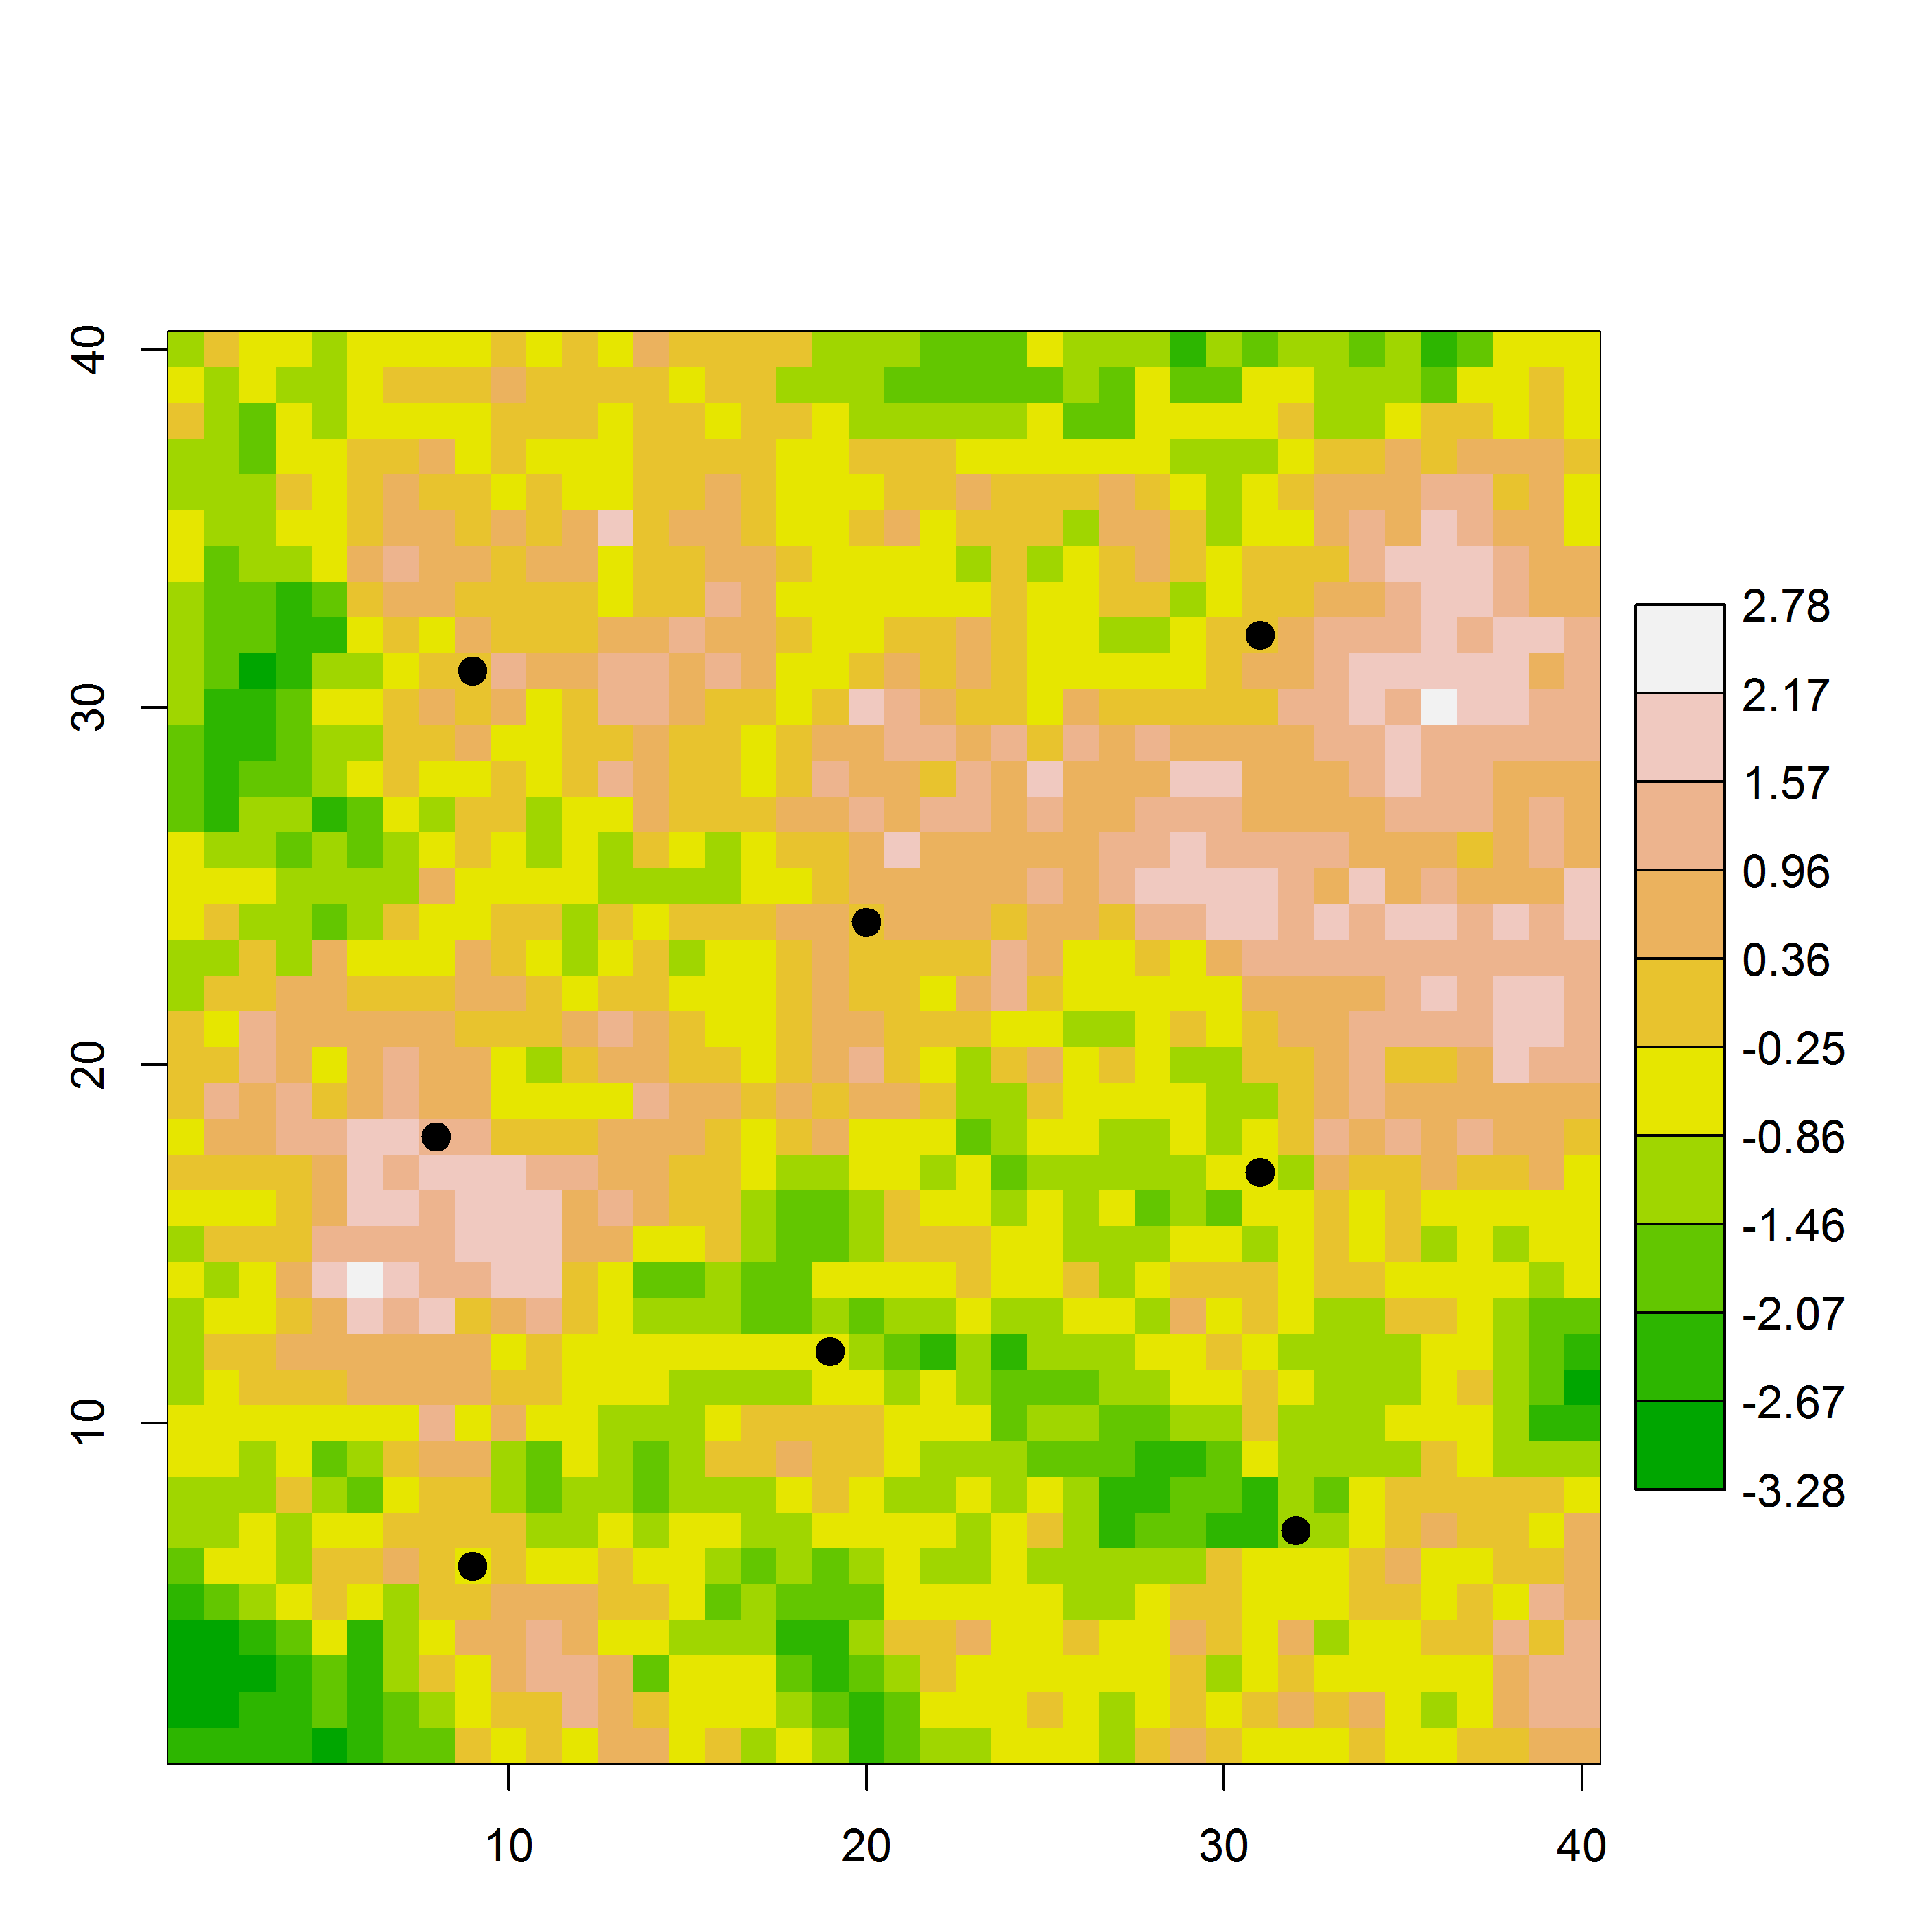
\includegraphics[width=4in,height=4in]{Ch10b/figs/habitat}
\caption{A habitat covariate. Home range centers for 8 individuals are
shown with black dots.}
\label{rsf.fig.habitat}
\end{figure}


\begin{figure}[htp]
\centering

\includegraphics[width=4in,height=4in]{Ch10b/figs/homeranges8}
\caption{Space usage patterns of 8 individuals under a space usage
  model that contains a single covariate (shown in
  Fig. \ref{rsf.fig.habitat}). 
\label{rsf.fig.homeranges}
\end{figure}





\subsection{Poisson use model}

A natural way to movitate this specific model is to
assume that individuals make a sequence of random resource selection
decisions so that the outcome of $n_{ij}$ are marginally {\it
  independent}, having a Poisson distribution:
\[
 n_{ij} \sim Poisson( \lambda_{ij})
\]
where
\[
 log(\lambda_{ij}) = a_{0}  + \alpha_{2} z(x)
\]
Therefore, the number of visits to any particular cell is affected by
the covariate $z(x)$ but has a baseline rate ($exp(a_{0})$) related to the amount
of movement, or number of selection decisions which is,
in a sense,
``up to the animal''. As such, the total sample size, among all
pixels, is a matter of how many choices, how much movement, the
individual is doing over some time interval.

\subsection{Thinning}

Suppose our sampling is imperfect so that we only observe a smaller
number of fixes than $n_{ij}$. As in sec. \ref{scr0.sec.implied}, we assume
\[
 m_{ij} \sim Bin(n_{ij}, \lambda_{0})
\]
in which case, marginally, $m_{ij}$ is also Poisson but with intensity
$log(\lambda_{0}) + a_{0}$ but we note that the RSF of the imperfect
coutns $m_{ij}$ is the same as the original RSF model for perfect
data. i.e., for ``truth''.
This is because if we remove $n_{ij}$ from this model by summing over
possible values, then the vector of ${\bf m}_{i}$ has a multinomial
with cell probabilities $\lambda_{0}\pi_{ij}$ and we see that
$\lambda_{0}$ cancels. 

%That is, 
%given our sequence of 
%independent Poisson random variables and we condition on their total,
%i.e., regard it as fixed, then we have the multinomial. In the
%multinomial we lose information about the intercept which in this case
%is ok because we only care about the interpretation of the resource
%selection model as a probability distribution and don't care about the
%basic rate of detection -- and it is a confounding of animal use and a
%fixed sampling intensity. 

In summary, if 
we conduct a telemetry study we observe ${\bf n}_{i}$, the $nG \times
1$ vector of pixel-counts for each individual $i=1,\ldots,N_{tel}$.
We declare these data to be ``resource-selection data'' which are
typical of the type used to estimate resource-selection functions
(RSFs) XXX REF XXXXX. Sometimes in RSF modeling activities people make believe they
have  continuous covariates and so the denominator in XXXX involves
some kind of integration over a distribution for the
covariate. However, in a discrete landscape, entertaining pdfs for the
covariates isn't necessary \citep{royle_etal:2012mee}. 


\subsection{SCR Data}

The key to combing RSF data with SCR data is to 
work with this underlying resource utilization process and formulate SCR
models in terms of that process. For SCR models it will serve as a
intermediate latent that we don't get to observe. We assume that,
fundamentally, both telemetered individuals and SCR individuals are
using space according to the same resourc selection model. The 
difference is that, for SCR data, we dissolve out most of the pixels
so that data are only recorded at a subsample of them.  

In other words, imagine that we have a sampling device, such as a
camera trap, in {\it every} pixel. If the device operates continually
then it is no different from a telemetry instrument, and if it
operates at some intermittently and does not expose the entire area of
each pixel then a reasonable model for this imperfect observation is
the ``thinned'' binomial model given above, where $\lambda_{0}$
represents the sampling effectiveness of the device. So we imagine
that the hypothetical perfect data from a camera trapping study are
the counts $m_{ij}$. 


With SCR data, under the Bernoulli model, 
 we only observe a random variable 
$y_{ijk} = 1$  if the individual $i$ visited the pixel
containing a trap and was detected. 
We imagine that $y$ is related to the latent variable $m$ being the
event $m>0$, which occurs with probability 
\[
 p_{ij} = 1-exp(- \lambda_{ij} p_{0} ) 
\]
we see that $p_{0}$ and a baseline rate of use  $exp(\beta_{0})$ are
all balled up together which makes sense. 
think of this as follows: we have some detector sitting there in a
pixel and we sample continuously and $p_{0}$ is the rate of encounter
given that an individuals visits a pixel. 


\section{The likelihood}

For sampling over $K$ periods the frequency of capture in each trap is
a binomial outcome
\[
 y_{ij} \sim Binomial(K; p_{ij})
\]
\[
 p_{ij} = 1-exp(- \lambda_{ij} p_{0} ) 
\]
and
\[
 \lambda_{ij} = \lambda_{0} exp(- \alpha_{1} D_{ij}^{2} + \alpha_{2}  z(x_{j}) )
\]
The likelihood for the SCR data, conditional on ${\bf s}_{i}$, is of
the form:
\begin{equation}
y_{ij}| {\bf s}_{i} \sim \mbox{Bin}(K, p_{\alpha}(D_{ij}; {\bm \alpha}))
\label{rsf.mle.eq.cond-on-s}
\end{equation}
For the random effect we have ${\bf s}_{i} \sim  \mbox{Unif}({\cal
  S})$.
The joint distribution of the data for individual $i$ is the product
of $J$ binomial terms (i.e., contributions from each of $J$ traps):
\[
  [{\bf y}_{i} | {\bf s}_{i} , \alpha] =
  \prod_{j=1}^{J} \mbox{Bin}(K, p_{\alpha}({\bf x}_{j},{\bf s}_{i}) )
\]
 The so-called marginal likelihood is computed by removing
${\bf s}_{i}$, by integration,  from the conditional-on-${\bf s}$
likelihood and regarding the {\it marginal} distribution of the data
as the likelihood. That
is, we compute:
\[
  [y|{\bm \alpha}] =
\int_{{\cal S}}  [ {\bf y}_{i} |{\bf s}_{i},{\bm \alpha}] g({\bf s}_{i}) d{\bf s}_{i}
\]
{\flushleft where}, under the uniformity assumption, we have
$g({\bf s}) = 1/||{\cal S}||$.
The joint likelihood for all $N$ individuals, 
is the product of $N$ such terms:
\[
{\cal L}({\bm \alpha} | {\bf y}_{1},{\bf y}_{2},\ldots, {\bf y}_{N}) = \prod_{i=1}^{N}
[{\bf y}_{i}|{\bm \alpha}]
\]

We have ${\bf m}_{i}$, the vector of pixel counts for a sample of
individuals from telemetry. Their likelihood contribution is
proportional to
\[
 logL = {\bf m}_{i}'{\bm \pi}_{i}
\]
where the element of ${\bm \pi}_{i}$ are of the form:
\[
 \pi_{i,j} = \frac{ exp( -\alpha_{1} D_{ij}^{2} -\alpha_{2} z(x) ) }
{ \sum_{x} exp(-\alpha_{1} D_{ij}^{2} -\alpha_{2} z(x))} 
\]
For telemetry data on a sample of individuals we  make one
simplifying assumption, which is that ${\bf s}$ is known for each
telemtered individual.  If we have a huge number of telemetry fixes
then this is probably reasonable.  In that case, we only have to
express the multinomial likelihood

The joint log-likelihood is the sum of those two pieces:
\[
{\cal L} = {\cal L}_{scr} + {\cal L}_{rsf}
\]
which we can maximize using standard methods. An exmaple is given here XXXXXXXXXXXXXXXXXXXXXXXXXXXXXX


Technical details for computing the likelihood and obtaining the MLEs
are given in XXXXXXX where we provide an ${\bf R}$ function to
evaluate the likelihood and obtain the MLEs.  A key practical detail
is that the likelihood here is formulated in terms of the parameter
$N$, the population size for the landscape defined by ${\cal
  S}$. Given ${\cal S}$, density is computed as $D({\cal S}) =
N/||{\cal S}||$. In our simulation study below we report $N$ as the
two are equivalent summaries of the data set once ${\cal S}$ is
defined.



\section{Illustration: Made up data}

Using patchy landscape covariate, as in Fig. XXXXX, for example we put
down a few hypotethcial activity centers and that produces the pictures.....



In this section we provide examples that we think are typical of how
cost-weighted distance models can be used in real capture-recapture
problems.  We define a $20 \times 20$ pixel landscape with 
extent = $[0.5, 4.5] \times [0.5, 4.5]$.  
%We define this landscape by
%a single covariate for determing the cost function, and we consider
%two specific covariates.
%purposes of our example, as a coarse landscape covariate, with pixels
%having some arbitrary scaling say, a $2 \times 2$ km resolution. Thus,
%the raster defines a landscape of $40 \times 40$ km and we suppose
We suppose that 16 camera traps are established at the integer coordinates
$(1,1), (1,2), \ldots, (4,4)$. We could think of this as a landscape
within which we're studying a population of ocelots, lynx or some
other cat.

For our analyses, cost is characterized by a single covariate 
and we consider two specific cases. First is an increasing trend from
the NW to the SE (''systematic landscape''), where $z(x)$ is defined as
$z(x) = r(x) + c(x)$ where $r(x)$ and $c(x)$ are just the row and
column, respectively, of the landscape.  This might define something
related to distance from an urban area or a gradient in habitat
quality due to land use, or environmental conditions such as
temperature or precipitation gradients.  In the second case we make up
a covariate by generating a field of spatially correlated noise to
emulate a typical patchy habitat covariate (''patchy landscape'') such as
tree or understory density. The two covariates are shown in
Fig. \ref{ecoldist.fig.raster100}, along with a sample realization of
$N=100$ individuals (left panel only).  For both covariates we use a
cost function in which transitions from pixel ${\bf x}$ to ${\bf x}'$
is given by:

\[
 log(cost({\bf x},{\bf x}'))=  \theta_2 \frac{z({\bf x}) + z({\bf x}')}{2}
\]

{\flushleft where} $\theta_2 = 1$ for our simulation.
When $\theta_2=0$ the
model reduces to one in which the cost of moving across each pixel is
constant, and therefore distance is Euclidean.


\section{Precision improvement}

Small simulation study -- ordinary SCR data with intense resource selection,

(1) how bad is the ordinary SCR model?

(2) how much does having 5 or 10 telemetered individuals provide?


\section{Summary and Outlook}


All published applications of SCR models to date have been based on
encounter probability models that are symmetric and stationary (do not
vary in space).


How animals use space and therefore how distance to a trap is
perceived by individuals is not something that can ever be known. We
can only ever conjure up models to describe this phenomenon and fit
those models to limited data on a sample of individuals during a
limited amount of time.  Here we have shown that there is hope to
estimate parameters, from capture-recapture data, that describe how
animals use space and thereby allow for irregular home range geometry
that is influenced by landscape structure.

Not surprisingly, our simulation study demonstrated
(Table 2) that the MLE of model parameters is
approximately unbiased in moderate sample sizes. Moreover, the effect
of ignoring ecological distance and using normal Euclidean distance in
the model for encounter probability, has the logical effect of causing
negative bias in estimates of $N$.  We expect this because the effect
is similar to failing to model heterogeneity. i.e., if we mis-specify
``model $M_h$'' \citep{otis_etal:1978} with ``model $M_0$''
\citep{otis_etal:1978} then we will expect to under-estimate $N$. So
the effect of mis-specifying the ecological distance metric with a
standard homogeneous Euclidean distance has the same effect. As a
practical matter, it stands to reason that many previous applications
of SCR models based on homogeneous distance metrics have under-stated
density of the focal population.

In our view, this bias is not really the most important reason to
consider models of ecological distance. Rather, inference about the
structure of ecological distance is fundamental to many problems in
applied and theoretical ecology related to modeling landscape
connectivity, corridor and reserve design, population viability
analysis, gene flow, and other phenomena.  Our new model allows
investigators to evaluate landscape factors that influence movement of
individuals over the landscape from non-invasively collected
capture-recapture data.  Therefore SCR models based on ecological
distance metrics might aid in understanding
aspects of space usage and movement in animal populations and, ultimately, in addressing conservation-related problems such as corridor design.

We considered inference for ecological distance models based on
marginal likelihood \citep{borchers_efford:2008}
(see Chapt. \ref{chapt.mle}).
In principle,
Bayesian analysis does not pose any unique challenges for this new
class of models, except that computing the cost-weighted distance is
computationally intensive.  So, having to do this at each iteration of
an MCMC algorithm may be impractical using existing algorithms.  A
related issue is that the size of the raster slows things down. For
very large rasters, even likelihood analysis can be computationally
challenging and methods for efficient calculation of the ecological
distance given the raster covariate(s) and parameters might be needed.





























